\documentclass{article}

\usepackage{defines}

\begin{document}

\tickettitle{13}{Понятие векторного произведения векторов. Лемма о построении. Четыре~свойства~векторного~произведения.}

\define{векторного произведения векторов}

\begin{minipage}{0.6\linewidth}
	Векторное произведение $\vec{a}$ на $\vec{b}$ обозначается\\
	как $[\vec{a},\vec{b}]$ или $\vec{a}\times\vec{b}$:
	\begin{enumerate}
		\item{}$|\vec{a}\times\vec{b}|:=|\vec{a}||\vec{b}|\sin\angle(\vec{a},\vec{b})$
		\item{}$(\vec{a}\times\vec{b})\perp\vec{a}\land(\vec{a}\times\vec{b})\perp\vec{b}$
		\item{}$(\vec{a},\vec{b},\vec{c})$ --- правая тройка
	\end{enumerate}
\end{minipage}%
\begin{minipage}{0.4\linewidth}
	\centering
	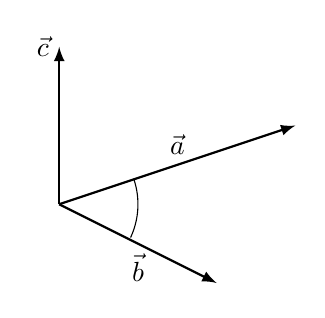
\begin{tikzpicture}
		\draw [-latex, thick] (0,0)--(3,1) node[midway, above] {$\vec{a}$};
		\draw [-latex, thick] (0,0)--(2,-1) node[midway, below] {$\vec{b}$};
		\draw [-latex, thick] (0,0)--(0,2) node[left] {$\vec{c}$};
		\draw [domain=-25:19] plot ({cos(\x)},{sin(\x)});
	\end{tikzpicture}
	\captionof{figure}{Векторное произведение}
\end{minipage}

\lemma[о построении]

$\vec{a}\nparallel\vec{e}\land|\vec{e}|=1$, тогда $[\vec{a},\vec{e}]=\lvec{OA''}$ можно найти следущим образом:
\begin{enumerate}
	\item{}Векторы $\vec{a}$ и $\vec{e}$ привести к общему началу $O$
	\item{}$\alpha:\alpha\perp\vec{e}$
\end{enumerate}

\end{document}
